\section{Analysis}
\label{sec:analysis}

\begin{table*}[!t]
\centering
\setlength{\tabcolsep}{4pt}
\resizebox{\textwidth}{!}{%
\begin{tabular}{l c c c c c c c c c c c c}
\toprule
& \multicolumn{2}{c}{\textbf{TriviaQA}}
& \multicolumn{2}{c}{\textbf{TruthfulQA}}
& \multicolumn{2}{c}{\textbf{MMLU-Pro}}
& \multicolumn{2}{c}{\textbf{GSM8K}}
& \multicolumn{2}{c}{\textbf{BBH}}
& \multicolumn{2}{c}{\textbf{Mean}} \\
\cmidrule(lr){2-3}\cmidrule(lr){4-5}\cmidrule(lr){6-7}\cmidrule(lr){8-9}\cmidrule(lr){10-11}\cmidrule(lr){12-13}
\textbf{Method}
  & ECE$\downarrow$ & AUROC$\uparrow$
  & ECE$\downarrow$ & AUROC$\uparrow$
  & ECE$\downarrow$ & AUROC$\uparrow$
  & ECE$\downarrow$ & AUROC$\uparrow$
  & ECE$\downarrow$ & AUROC$\uparrow$
  & ECE$\downarrow$ & AUROC$\uparrow$ \\
\midrule
Scalar~+~GBT       & 11.15 {\scriptsize $\pm$ 4.43} & 80.28 {\scriptsize $\pm$ 4.95} & 23.50 {\scriptsize $\pm$ 12.68} & 70.46 {\scriptsize $\pm$ 2.14} & 16.39 {\scriptsize $\pm$ 4.04} & 60.73 {\scriptsize $\pm$ 4.28} & 10.14 {\scriptsize $\pm$ 3.84} & 80.58 {\scriptsize $\pm$ 2.49} & 13.33 {\scriptsize $\pm$ 4.22} & 62.48 {\scriptsize $\pm$ 2.54} & 14.90 {\scriptsize $\pm$ 1.73} & 70.91 {\scriptsize $\pm$ 2.54} \\
GraphCal           & 11.93 {\scriptsize $\pm$ 4.66} & 80.13 {\scriptsize $\pm$ 5.01} & 34.15 {\scriptsize $\pm$ 9.54} & 63.51 {\scriptsize $\pm$ 2.89} & 14.41 {\scriptsize $\pm$ 2.17} & 54.79 {\scriptsize $\pm$ 5.86} & 19.59 {\scriptsize $\pm$ 6.43} & 80.92 {\scriptsize $\pm$ 6.54} & 20.05 {\scriptsize $\pm$ 4.09} & 70.62 {\scriptsize $\pm$ 3.60} & 20.03 {\scriptsize $\pm$ 1.87} & 70.00 {\scriptsize $\pm$ 2.40} \\
DiscoUQ-LLM       & 12.52 {\scriptsize $\pm$ 5.24} & 82.60 {\scriptsize $\pm$ 4.90} & 24.42 {\scriptsize $\pm$ 13.93} & 71.78 {\scriptsize $\pm$ 3.72} & 16.83 {\scriptsize $\pm$ 4.67} & 59.37 {\scriptsize $\pm$ 7.95} & 10.09 {\scriptsize $\pm$ 4.12} & \textbf{84.59 {\scriptsize $\pm$ 3.95}} & 15.25 {\scriptsize $\pm$ 4.40} & 63.00 {\scriptsize $\pm$ 3.58} & 15.82 {\scriptsize $\pm$ 8.45} & 72.27 {\scriptsize $\pm$ 11.32} \\
\rowcolor[RGB]{222,230,241}
\textbf{\methodname{} (ours)}
                  & \textbf{4.63 {\scriptsize $\pm$ 0.71}}  & \textbf{85.74 {\scriptsize $\pm$ 1.41}}
                  & \textbf{8.70 {\scriptsize $\pm$ 1.84}}  & \textbf{79.59 {\scriptsize $\pm$ 4.67}}
                  & \textbf{11.19 {\scriptsize $\pm$ 1.29}} & \textbf{76.67 {\scriptsize $\pm$ 3.63}}
                  & \textbf{1.89 {\scriptsize $\pm$ 1.31}}  & 80.39 {\scriptsize $\pm$ 5.75}
                  & \textbf{6.38 {\scriptsize $\pm$ 1.38}}  & \textbf{88.67 {\scriptsize $\pm$ 1.12}}
                  & \textbf{6.56 {\scriptsize $\pm$ 0.68}}  & \textbf{82.21 {\scriptsize $\pm$ 1.84}} \\
\bottomrule
\end{tabular}%
}
\vspace{-5pt}
\caption{\textbf{Leave-one-topology-out (LOTO) generalization.}
ECE ($\downarrow$) and AUROC ($\uparrow$), mean over the 5
held-out-topology folds. Trained calibrators only.}
\label{tab:main-loto}
\vspace{-15pt}
\end{table*}

\begin{table}[!h]
\centering
\setlength{\tabcolsep}{4pt}
\resizebox{\columnwidth}{!}{%
\begin{tabular}{l c c c}
\toprule
\textbf{Variant}                          & \textbf{ECE} $\downarrow$
                                            & \textbf{AUROC} $\uparrow$
                                            & \textbf{AUARC} $\uparrow$ \\
\midrule
\rowcolor{gray!20}
\multicolumn{4}{c}{\textit{Scalar-summary baselines}}\\
Scalar summaries + LR                & $8.03${\scriptsize$\pm0.35$}
                                             & $74.12${\scriptsize$\pm1.24$}
                                             & $71.64${\scriptsize$\pm0.69$} \\
Scalar summaries + GBT                & $7.99${\scriptsize$\pm0.95$}
                                             & $74.78${\scriptsize$\pm1.32$}
                                             & $72.70${\scriptsize$\pm0.50$} \\
\midrule
\rowcolor{gray!20}
\multicolumn{4}{c}{\textsc{CAGE-Cal} incremental variants}\\
Observed graph encoder only               & $6.97${\scriptsize$\pm0.28$}
                                             & $81.25${\scriptsize$\pm0.88$}
                                             & $75.61${\scriptsize$\pm0.13$} \\
\,\,+ Iid counterfactual tower                  & $6.78${\scriptsize$\pm0.33$}
                                             & $81.89${\scriptsize$\pm1.47$}
                                             & $75.79${\scriptsize$\pm0.24$} \\
% \rowcolor[RGB]{222,230,241}
% \multicolumn{1}{c}{$\Delta$ vs. previous}
% & {$-0.19$}
% & {$+0.64$}
% & {$+0.18$} \\
\,\,+ Group-level hyperedge stream                      & $6.75${\scriptsize$\pm0.37$}
                                             & $82.56${\scriptsize$\pm1.27$}
                                             & $76.08${\scriptsize$\pm0.38$} \\
% \rowcolor[RGB]{222,230,241}
% \multicolumn{1}{c}{$\Delta$ vs. previous}
% & {$-0.03$}
% & {$+0.67$}
% & {$+0.29$} \\

\,\,+ Calibration-aware objective (full)         & \textbf{5.56{\scriptsize$\pm0.03$}}
                                             & \textbf{83.61{\scriptsize$\pm1.34$}}
                                             & \textbf{76.47{\scriptsize$\pm0.37$}} \\
\rowcolor[RGB]{222,230,241}
\multicolumn{1}{c}{$\Delta$ vs. base}
& {$-1.41$}
& {$+2.36$}
& {$+0.86$} \\
\bottomrule
\end{tabular}%
}
\vspace{-5pt}
\caption{\textbf{Component ablation of \textsc{CAGE-CAL}}, averaged over 25 in-distribution cells 
(percent, mean $\pm$ std over 3 rollouts). 
$\Delta$ rows show absolute changes from the previous variant in percentage points. 
LR and GBT denote logistic regression and gradient-boosted trees.}
\label{tab:ablation}
\vspace{-15pt}
\end{table}




\subsection{Component Ablation}
\label{sec:ablation}

Table~\ref{tab:ablation} ablates the main components of \methodname{}. 
Scalar-summary baselines compress each panel into fixed statistics and remain far below graph-based variants, with the stronger GBT head reaching only $74.78$ AUROC and $72.70$ AUARC. 
The observed graph encoder raises AUROC to $81.25$, showing that panel reliability depends on relational structure beyond aggregate vote and confidence summaries. 
Adding the IID counterfactual tower further improves AUROC by $0.64$ points, while the group-level hyperedge stream adds another $0.67$ points by capturing shared family, role, answer-cluster, and exposure effects. 
The calibration-aware objective gives the largest ECE reduction, from $6.75$ to $5.56$, without sacrificing ranking quality. 
Overall, the gains come from modeling a counterfactual dependence shift, not from simply adding a stronger prediction head.

\subsection{Generalization to Held-Out Topologies}
\label{sec:loto}

We test topology generalization with leave-one-topology-out evaluation. 
Each fold removes one topology from both training and validation, and evaluates the calibrator on that unseen topology.
As shown in Table~\ref{tab:main-loto}, \methodname{} remains stable under this shift. 
Its mean AUROC is $82.21$, close to the in-distribution result of $83.61$, and its mean ECE rises only from $5.56$ to $6.56$. 
By comparison, DiscoUQ-LLM reaches $72.27$ mean AUROC and $15.82$ mean ECE. 
This indicates that scalar disagreement features do not transfer as well when the communication structure changes.
The result supports the relational design of \methodname{}. 
Rather than relying on a topology label, it uses communication edges, local failure correlations, answer clusters, and group-level dependency units. 
These features are defined for any topology, allowing the calibration rule to transfer to unseen communication structures.


\subsection{Correcting the Two Failure Modes}
\label{sec:failure_diagnostics}

Figure~\ref{fig:failure_fix} tests whether \methodname{} corrects the two calibration failures identified earlier. 
In Mode A, iid/TriviaQA, plurality share is under-confident because wrong answers are dispersed across weak clusters. 
In Mode B, chain/TruthfulQA, plurality share is over-confident because communication can concentrate agents on the same wrong answer. 
In both cases, \methodname{} moves the reliability curve closer to the perfect calibration line. 
Thus, the same vote share can receive different confidence depending on how the agreement or disagreement was formed.
\begin{figure}[!t]
  \centering
  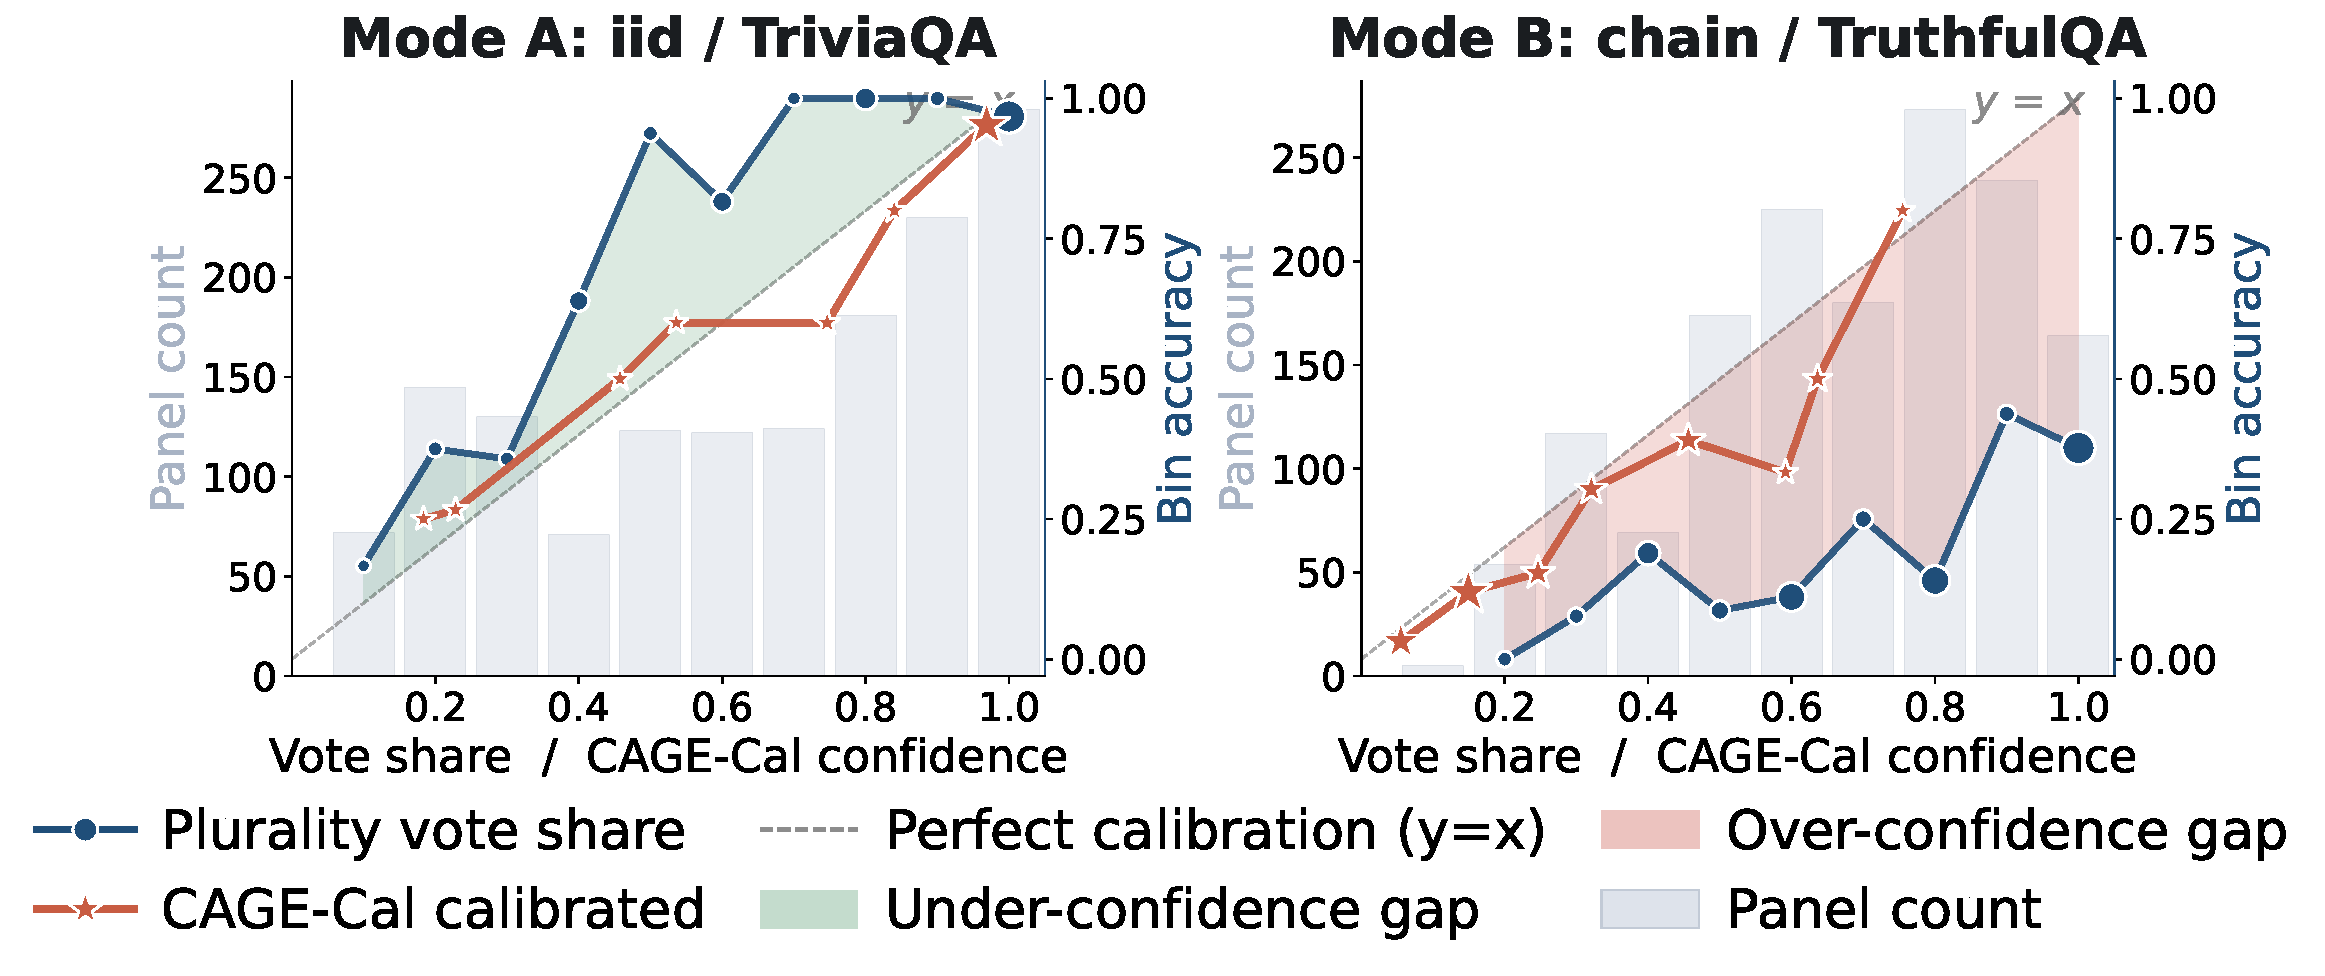
\includegraphics[width=\columnwidth]{figures/fig_failure_fix.pdf}
  \vspace{-20pt}
  \caption{\textbf{Failure-mode correction.} 
Bars show panel counts, and curves show empirical bin accuracy when examples are binned by plurality share or by \methodname{} confidence. 
\methodname{} reduces under-confidence in Mode A and over-confidence in Mode B.
}
  \label{fig:failure_fix}
\vspace{-15pt}
\end{figure}